%% Based on a TeXnicCenter-Template by Gyorgy SZEIDL.
%%%%%%%%%%%%%%%%%%%%%%%%%%%%%%%%%%%%%%%%%%%%%%%%%%%%%%%%%%%%%

%----------------------------------------------------------
%
\documentclass{report}%
%
%----------------------------------------------------------
% This is a sample document for the standard LaTeX Report Class
% Class options
%       --  Body text point size:
%                        10pt (default), 11pt, 12pt
%       --  Paper size:  letterpaper (8.5x11 inch, default)
%                        a4paper, a5paper, b5paper,
%                       legalpaper, executivepaper
%       --  Orientation (portrait is the default):
%                       landscape
%       --  Printside:  oneside (default), twoside
%       --  Quality:    final (default), draft
%       --  Title page: titlepage, notitlepage
%       --  Columns:    onecolumn (default), twocolumn
%       --  Start chapter on left:
%                       openright(no), openany (default)
%       --  Equation numbering (equation numbers on right is the default)
%                       leqno
%       --  Displayed equations (centered is the default)
%                       fleqn (flush left)
%       --  Open bibliography style (closed bibliography is the default)
%                       openbib
% For instance the command
%          \documentclass[a4paper,12p,leqno]{report}
% ensures that the paper size is a4, fonts are typeset at the size 12p
% and the equation numbers are on the left side.
%
\usepackage{amsmath}%
\usepackage{amsfonts}%
\usepackage{amssymb}%
\usepackage{graphicx}
%----------------------------------------------------------
\usepackage{url}
\usepackage{tabularx}
%\usepackage{tablefootnote}
\usepackage[square,sort,comma,numbers]{natbib}
\usepackage{chapterbib}
\usepackage{hyperref}
\usepackage{url}
\usepackage{doi}
\usepackage{listings}
\usepackage{color}
%----------------------------------------------------------
% Define colors:
\definecolor{dkgreen}{rgb}{0,0.6,0}
\definecolor{gray}{rgb}{0.5,0.5,0.5}
\definecolor{mauve}{rgb}{0.58,0,0.82}
% Define language
\lstdefinelanguage{torxakis}
{
  % list of keywords
  morekeywords={
    PROCDEF,
    FUNCDEF
  },
  sensitive=false, % keywords are not case-sensitive
  morecomment=[l]{//}, % l is for line comment
  morecomment=[s]{/*}{*/}, % s is for start and end delimiter
  morestring=[b]" % defines that strings are enclosed in double quotes
}
% Define environment:
\lstset{frame=tb,
  language=torxakis,
  aboveskip=3mm,
  belowskip=3mm,
  showstringspaces=false,
  columns=flexible,
  basicstyle={\small\ttfamily},
  numbers=none,
  numberstyle=\tiny\color{gray},
  keywordstyle=\color{blue},
  commentstyle=\color{dkgreen},
  stringstyle=\color{mauve},
  breaklines=true,
  breakatwhitespace=true,
  tabsize=3
}
%----------------------------------------------------------
\newcommand{\txs}{TorXakis}
\newcommand{\mcrl}{mCRL2}
\newcommand{\inlinecode}[1]{{\lstinline[language=torxakis]{#1}}}
\newcommand{\istep}{\texttt{ISTEP}}
\newcommand{\cistep}{\texttt{CISTEP}}
\newcommand{\true}{\textbf{true}}
\newcommand{\false}{\textbf{false}}
\newcommand{\labeledas}[1]{labeled as `#1'}
\newcommand{\labeledaseither}[2]{labeled as `#1' or `#2'}
\newcommand{\removelabelfrom}[1]{remove the label `#1' from}
\newcommand{\sortof}[1]{\text{sort}(#1)}
\newcommand{\flsortof}[1]{\text{flsort}(#1)}
%----------------------------------------------------------
\setlength\parindent{0pt}
%----------------------------------------------------------
%\makeatletter
%\newcommand\footnoteref[1]{\protected@xdef\@thefnmark{\ref*{#1}}\@footnotemark}
%\makeatother
%----------------------------------------------------------
\newtheorem{theorem}{Theorem}
\newtheorem{acknowledgement}[theorem]{Acknowledgement}
\newtheorem{algorithm}[theorem]{Algorithm}
\newtheorem{axiom}[theorem]{Axiom}
\newtheorem{case}[theorem]{Case}
\newtheorem{claim}[theorem]{Claim}
\newtheorem{conclusion}[theorem]{Conclusion}
\newtheorem{condition}[theorem]{Condition}
\newtheorem{conjecture}[theorem]{Conjecture}
\newtheorem{corollary}[theorem]{Corollary}
\newtheorem{criterion}[theorem]{Criterion}
\newtheorem{definition}[theorem]{Definition}
\newtheorem{example}[theorem]{Example}
\newtheorem{exercise}[theorem]{Exercise}
\newtheorem{lemma}[theorem]{Lemma}
\newtheorem{notation}[theorem]{Notation}
\newtheorem{problem}[theorem]{Problem}
\newtheorem{proposition}[theorem]{Proposition}
\newtheorem{remark}[theorem]{Remark}
\newtheorem{solution}[theorem]{Solution}
\newtheorem{summary}[theorem]{Summary}
\newenvironment{proof}[1][Proof]{\textbf{#1.} }{\ \rule{0.5em}{0.5em}}
%----------------------------------------------------------
\begin{document}

\title{LPE operations}
\author{Djurre van der Wal}
\date{\today}
\maketitle
\tableofcontents

\chapter{Getting started}

\section{Introduction}

\txs{} offers several techniques to symbolically manipulate \txs{} models.
This section gives an overview of how to get started with these techniques.

\section{Installation}

\begin{enumerate}
\item Download \texttt{stack} from
\begin{align*}
\texttt{https://docs.haskellstack.org/en/stable/README/}
\end{align*}

and install it.

\item Download and install an SMT solver such as
\begin{align*}
\texttt{Z3 version 4.8.3 - 64 bit - build hashcode cf4bf7b591b6}
\end{align*}

Add the binaries of the SMT solver to \texttt{PATH}.
\item Clone the \texttt{develop} branch from
\begin{align*}
\texttt{https://github.com/TorXakis/TorXakis}
\end{align*}
\item In a terminal, navigate to the repository directory and run
\begin{itemize}
\item \texttt{stack setup}
\item \texttt{stack -v --profile build}
\end{itemize}
\item The \txs{} binaries can be found in
\begin{align*}
\texttt{/.stack-work/install/23f9efff/bin}
\end{align*}

in the repository directory (the \texttt{23f9efff} hash is build-dependent).

Add the binaries to \texttt{PATH}.
\end{enumerate}

\section{Starting \txs{}} \label{starttxs}

\begin{enumerate}
\item Make it so that \texttt{txsserver.exe} and \texttt{torxakis.exe} are in \texttt{PATH}.
\item Start two terminals, one for the \txs{} server and one for the \txs{} client -- this has the advantage of any errors that occur on the server-side to be visible.
\item In both terminals, navigate to the directory with a \txs{} specification file (such as \texttt{example.txs}).
\item In one terminal, run \texttt{txsserver --no-smt-log 50001} where the number \texttt{50001} is the port number that the \txs{} server will listen for clients.
\item In the other terminal, run \texttt{torxakis 50001 example.txs}.
\end{enumerate}

\section{Process linearization} \label{processlinearization}

The symbolic manipulation of \txs{} models requires the processes that underlie those models to be in \emph{LPE form} (see \ref{lpeform}).
To make a \txs{} process linear in practice, do the following:

\begin{enumerate}
\item Start \txs{} (see \ref{starttxs}).
\item Run
\begin{align*}
\texttt{lpe Model}
\end{align*}

in the client terminal, where \texttt{Model} is the name of the model in the \txs{} specification file.
\txs{} will attempt to linearize the processes that underlie that model.

Note that not all \txs{} models are linearizable.
For those models, the \texttt{lpe} command will fail, with an error reported in the server terminal.
\item If successful, the \texttt{lpe} command prints the name of a new \txs{} model that was created.
This model can be manipulated symbolically (see \ref{modelmanipulation}).
\end{enumerate}

\section{Model manipulation} \label{modelmanipulation}

After \ref{starttxs} and \ref{processlinearization}, symbolic manipulation of a \txs{} model can begin.
To do this, use the \texttt{lpeop} command in the client terminal.

The \texttt{lpeop} command has 3 space-separated arguments. In order, these arguments are:

\begin{itemize}
\item A chain of LPE operations.
LPE operations are represented by their name, such as \texttt{cstelm} or \texttt{loop} (see \ref{lpeoperations}).
These names are separated by the symbol \texttt{->}.

LPE operations in the chain are executed from left to right, passing their output to the next LPE operation as input.
If a problem occurs, the process ends immediately.
Otherwise, the final output model is saved as a new model.
\item The name of the input model.
The process that underlies the input model should be in LPE form (see \ref{lpeform}).
\item A base name \textit{base} for generated output.
The name is primarily used for the output model (if any), the underlying process of which is in LPE form.
However, LPE operations may adopt the name for their own purposes.
The \texttt{export} operation, for example, will create a file by that name with the \texttt{.txs} extension.

It is possible to use the \texttt{\%i} token in the base name.
This will insert the current counter value into the name.
Use the \texttt{inc} command to increase the counter (which starts at 1).
\end{itemize}

\subsection{Examples TODO}

TODO

\section{Unit tests}

\begin{enumerate}
\item In a terminal, navigate to the repository directory.
\item Execute \texttt{stack -v --profile test lpeops}.
\end{enumerate}

\section{Benchmarks}

\subsection{Generation (Windows OS only)}
First, benchmark files must be generated.
This is done via script.

\begin{enumerate}
\item Navigate to \texttt{/examps} and open the file
\begin{align*}
\texttt{generateBenchmarkData.bat}
\end{align*}

\item Change \texttt{TXSDIR} to the directory where the \txs{} source files are located.
Among others, it should contain the following sub-directories:
\begin{center}
\texttt{examps} \\
\texttt{sys} \\
\texttt{test}
\end{center}

\item In order to perform different benchmark measurements, change the contents of the function \texttt{:WriteCommands} (line 104, in particular, describes how the model should be produced that is compared to the original model and the linearized model).

\item Run \texttt{generateBenchmarkData.bat} and wait for it to finish.
\end{enumerate}

\subsection{Execution}
The main benchmark file of \txs{},
\begin{align*}
\texttt{/test/sqatt/src/Benchmarks/All.txs}
\end{align*}

has been changed, and so the benchmark for LPE operations is started in the same way as the original benchmark:

\begin{enumerate}
\item In a terminal, navigate to \texttt{/test/sqatt} in the repository directory.
\item Execute
\begin{align*}
\texttt{stack -v --profile bench --ba "--output data.html"}
\end{align*}

\item Wait for the benchmark to finish.
If there are no failures, the benchmark results will be exported to \texttt{data.html}.
\end{enumerate}


\chapter{LPE structure}

\section{Introduction}
The LPE operations that are described in this document (see \ref{lpeoperations}) require a \txs{} model as input of which the process is in \emph{linear process equation} (LPE) \emph{form}.
Many, but not all \txs{} processes can be transformed to LPE form using the \texttt{lpe} command of \txs{}.

\section{LPE form} \label{lpeform}

A \txs{} process
\begin{align*}
\texttt{ProcDef} \; [C_1 :: K_1, \cdots{}, C_n :: K_n] \; [p_1 :: T_1, \cdots{}, p_k :: T_k] \; b_\textit{LPE}
\end{align*}

that is identified by $P$ is said to be a in \emph{LPE form} if $b_\textit{LPE}$ follows the grammar of $\textit{LPEBody}$ below:
\begin{align*}
\textit{LPEBody} &::= \textit{ChoiceSmd} \\
\textit{ChoiceSmd} &::= \texttt{Choice} \; [ \;\! \textit{ActionSmd}, \cdots{}, \textit{ActionSmd} \; ] \\
\textit{ActionSmd} &::= \texttt{ActionPref} \; \textit{ActOffer} \; \textit{ProcInst} \\
\textit{ActOffer} &::= \texttt{ActOffer} \; \textit{ChanOffers} \;\; [ \; h_1, \cdots{}, h_z \; ] \; \textit{VExpr} \\
\textit{ChanOffers} &::= [ \;\! \textit{ChanOffer}, \cdots{}, \textit{ChanOffer} \; ] \\
\textit{ChanOffer} &::= \textit{ChanId} \;\; [\texttt{Quest} \; x_1, \cdots{}, \texttt{Quest} \; x_m] \\
\textit{ChanId} &::= C_1 \;| \cdots{} |\; C_n \;|\; \texttt{ISTEP} \;|\; \texttt{CISTEP} \\
\textit{ProcInst} &::= \texttt{ProcInst} \; P \; \; [ \; C_1, \cdots{}, C_n \; ] \; [\;\!\textit{VExpr}, \cdots{}, \textit{VExpr} \; ]
\end{align*}

Note that
\begin{itemize}
\item $b_\textit{LPE}$ should comply with traditional \txs{} requirements.
More precisely, the communication variables $\{ x_1, \cdots{}, x_m \}$ must match the signature of the \textit{ChanId} channel that occurs in the same rule; and the number of \textit{VExpr}s in the \textit{ProcInst} rule must be equal to $k$ and their sorts must match $[T_1, \cdots{}, T_k]$.
\item it must be the case that the channels that are used in a summand are either all input channels or all output channels.
\item per summand, it must be the case that
\begin{align*}
|\; \{ h_1, \cdots{}, h_z \} \cup \{ x_1, \cdots{}, x_m \} \; | &= z + m \\
(\{ h_1, \cdots{}, h_z \} \cup \{ x_1, \cdots{}, x_m \}) \cap \{ p_1, \cdots{}, p_k \} &= \emptyset{}
\end{align*}
\end{itemize}

\section{Restricted LPE form} \label{restrictedlpeform}

In actuality, it is convenient that processes have a form that is even more restrictive than the LPE form discussed in \ref{lpeform}.
The form is the same as before, except for the \textit{ActOffer} and \textit{ChanOffers} rules, which change to
\begin{align*}
\textit{ActOffer} &::= \texttt{ActOffer} \; \textit{ChanOffers} \;\; [\;] \; \textit{VExpr} \\
\textit{ChanOffers} &::= [ \;\! \textit{ChanOffer} \; ]
\end{align*}

In short, hidden variables are no longer permitted, and there must be exactly one \textit{ChanOffer} per summand.

A process that is in LPE form can be converted to restricted LPE form in a way that is reversible.
First, a more precise definition of the format of \txs{} models is required.

Let the form of a \txs{} model $M$ be
\begin{align*}
\texttt{ModelDef} \; [I_1, \cdots{}, I_m] \; [O_1, \cdots{}, O_n] \; b_\textit{inst}
\end{align*}

where

\begin{itemize}
\item $I_1, \cdots{}, I_m$ are all single input channels;
\item $O_1, \cdots{}, O_n$ are all single output channels;
\item $b_\text{\textit{inst}}$ has the form
\begin{align*}
\texttt{ProcInst} \; P \; [D_1, \cdots{}, D_{m+n}] \; [v_I(p_1), \cdots{}, v_I(p_k)]
\end{align*}

such that
\begin{align*}
\{ I_1, \cdots{}, I_m \}, \{ O_1, \cdots{}, O_n \} \subseteq \{ D_1, \cdots{}, D_{m+n} \}
\end{align*}

and
\begin{align*}
\{ I_1, \cdots{}, I_m \} \cap \{ O_1, \cdots{}, O_n \} = \emptyset{}
\end{align*}

\item the \txs{} process that is identified by $P$ is
\begin{align*}
\texttt{ProcDef} \; [C_1 :: K_1, \cdots{}, C_{m+n} :: K_{m+n}] \; [p_1 :: T_1, \cdots{}, p_k :: T_k] \; b_\textit{LPE}
\end{align*}
such that
\begin{align*}
\sortof{C_i} = \sortof{D_i} = K_i &\text{ for all } i \in [1, \cdots{}, m+n] \\
\sortof{v_I(p_i)} = T_i &\text{ for all } i \in [1, \cdots{}, k]
\end{align*}

and such that $b_\textit{LPE}$ follows the parametrized grammar of $\textit{LPEBody}$ below:
\begin{align*}
\textit{LPEBody} &::= \textit{ChoiceSmd} \\
\textit{ChoiceSmd} &::= \texttt{Choice} \; [ \;\! \textit{ActionSmd}(1), \cdots{}, \textit{ActionSmd}(s) \; ] \\
\textit{ActionSmd}(i) &::= \texttt{ActionPref} \; \textit{ActOffer}(i) \; \textit{ProcInst}(i) \\
\textit{ActOffer}(i) &::= \texttt{ActOffer} \; \textit{ChanOffers}(i) \; [ \; h_i(1), \cdots{}, h_i(z_i) \; ] \; g_i \\
\textit{ChanOffers}(i) &::= [ \;\! \textit{ChanOffer}_i(1), \cdots{}, \textit{ChanOffer}_i(m_i) \; ] \\
\textit{ChanOffer}_i(j) &::= c_i(j) \;\; [\texttt{Quest} \; x_{i,j}(1), \cdots{}, \texttt{Quest} \; x_{i,j}(|\flsortof{c_i(j)}|)] \\
\textit{ProcInst}_i(j) &::= \texttt{ProcInst} \; P \; \; [ \; C_1, \cdots{}, C_{m+n} \; ] \; [\;\!v_i(p_1), \cdots{}, v_i(p_k) \; ]
\end{align*}

where

\begin{itemize}
\item $s$ is the number of summands of $P$;
\item $h_i(j)$ is the $j$th hidden variable of the $i$th summand of $P$;
\item $z_i \geq 0$ is the number of hidden variables of the $i$th summand of $P$;
\item $g_i$ is the guard of the $i$th summand of $P$;
\item $m_i \geq 0$ is the number of channels over which the $i$th summand of $P$ communicates;
\item $c_i(j)$ is the $j$th channel over which the $i$th summand of $P$ communicates;
\item $\text{fl}(S_1 \; \texttt{\#\#} \cdots{} \texttt{\#\#} \; S_q) = [S_1, \cdots{}, S_q]$ for some $q > 0$;
\item $x_{i,j}(e)$ is the $e$th parameter that the $i$th summand of $P$ uses to communicate over channel $c_i(j)$;
\item $v_i(p)$ is an expression that defines the new value of parameter $p$ of $P$ after the application of summand $s_i$.
\end{itemize}
\end{itemize}

Define a \emph{channel signature} as a pair $(C, S)$ where $C$ is an ordered list of channels and $S$ is an ordered list of sorts, and define a function $\tau$ that yields the channel signature of the $i$th summand of $P$, namely $s_i$:
\begin{align*}
\tau(s_i) = (&[ c_i(1), \cdots{}, c_i(m_i)], \\
&[\flsortof{c_i(1)}, \cdots{}, \flsortof{c_i(m_i)}, \sortof{h_i(1)}, \cdots{}, \sortof{h_i(z_i)}])
\end{align*}

Also define an injective function $\theta(T)$ that maps channel signatures of the form
\begin{align*}
T = (C, [S_1, \cdots{}, S_{m_i+z_i}])
\end{align*}

to a fresh, uniquely named channel with sort $S_1 \; \texttt{\#\#} \cdots{} \texttt{\#\#} \; S_{m_i+z_i}$.

Given these definitions, do the following:

\begin{enumerate}
\item For each summand $s_i$, compute $\tau(s_i)$.
Add the result to a set $\Sigma_I$ if summand $s_i$ contains input actions, or add the result to a set $\Sigma_O$ if summand $s_i$ contains output actions (only one of these can be true).

\item Compute $\Omega_I = \{ \; (\sigma, \theta(\sigma)) \;|\; \sigma \in \Sigma_I \; \}$ and $\Omega_O = \{ \; (\sigma, \theta(\sigma)) \;|\; \sigma \in \Sigma_O \; \}$.

\item Compute $\Theta = [ \; \Theta_1, \cdots{}, \Theta_t \; ] = [ \; b \;|\; (a, b) \in \Omega_I \cup \Omega_O \; ]$.

\item For each summand $s_i$, look up a pair $(a, b) \in \Omega_I \cup \Omega_O$ so that $a = \tau(s_i)$.
There is exactly one such pair.
Change the form of $s_i$ to
\begin{align*}
\textit{ActionSmd}(i) &::= \texttt{ActionPref} \; \textit{ActOffer}(i) \; \textit{ProcInst}(i) \\
\textit{ActOffer}(i) &::= \texttt{ActOffer} \; \textit{ChanOffers}(i) \;\; [ \; ] \;\; g_i \\
\textit{ChanOffers}_i &::= [ \; b \;\; [ \;\! \textit{ChanOffer}_i(1), \cdots{}, \textit{ChanOffer}_i(m_i), \\
&\qquad \qquad \qquad \texttt{Quest} \; h_i(1), \cdots{}, \texttt{Quest} \; h_i(z_i) \; ] \; ] \\
\textit{ChanOffer}_i(j) &::= \texttt{Quest} \; x_{i,j}(1), \cdots{}, \texttt{Quest} \; x_{i,j}(|\flsortof{c_i(j)}|) \\
\textit{ProcInst}_i(j) &::= \texttt{ProcInst} \; P \; \; [ \; \Theta_1, \cdots{}, \Theta_t \; ] \; [\;\!v_i(p_1), \cdots{}, v_i(p_k) \; ]
\end{align*}

\item Change the definition of $P$ to
\begin{align*}
\texttt{ProcDef} \; [\Theta_1 :: \sortof{\Theta_1}, \cdots{}, \Theta_t :: \sortof{\Theta_t}] \; [p_1 :: T_1, \cdots{}, p_k :: T_k] \; b_\textit{LPE}
\end{align*}

\item Change the definition of $M$ to
\begin{align*}
\texttt{ModelDef} \; [ \; b \;|\; (a, b) \in \Omega_I \; ] \; [ \; b \;|\; (a, b) \in \Omega_O \; ] \; b_\textit{inst}
\end{align*}

where
\begin{align*}
b_\textit{inst} = \texttt{ProcInst} \; P \; [\Theta_1, \cdots{}, \Theta_t] \; [v_I(p_1), \cdots{}, v_I(p_k)]
\end{align*}
\end{enumerate}

Given $\Omega_I$ and $\Omega_O$, how to reverse the conversion above should be obvious.

\section{Data structure}

The implementation stores a \txs{} model that is in LPE form in a dedicated data structure before any of the techniques that are described in this document are applied.
A visual representation of this data structure can be found in Figure~\ref{lpedatastructure:fig}.

\begin{figure}[!ht]
\begin{center}
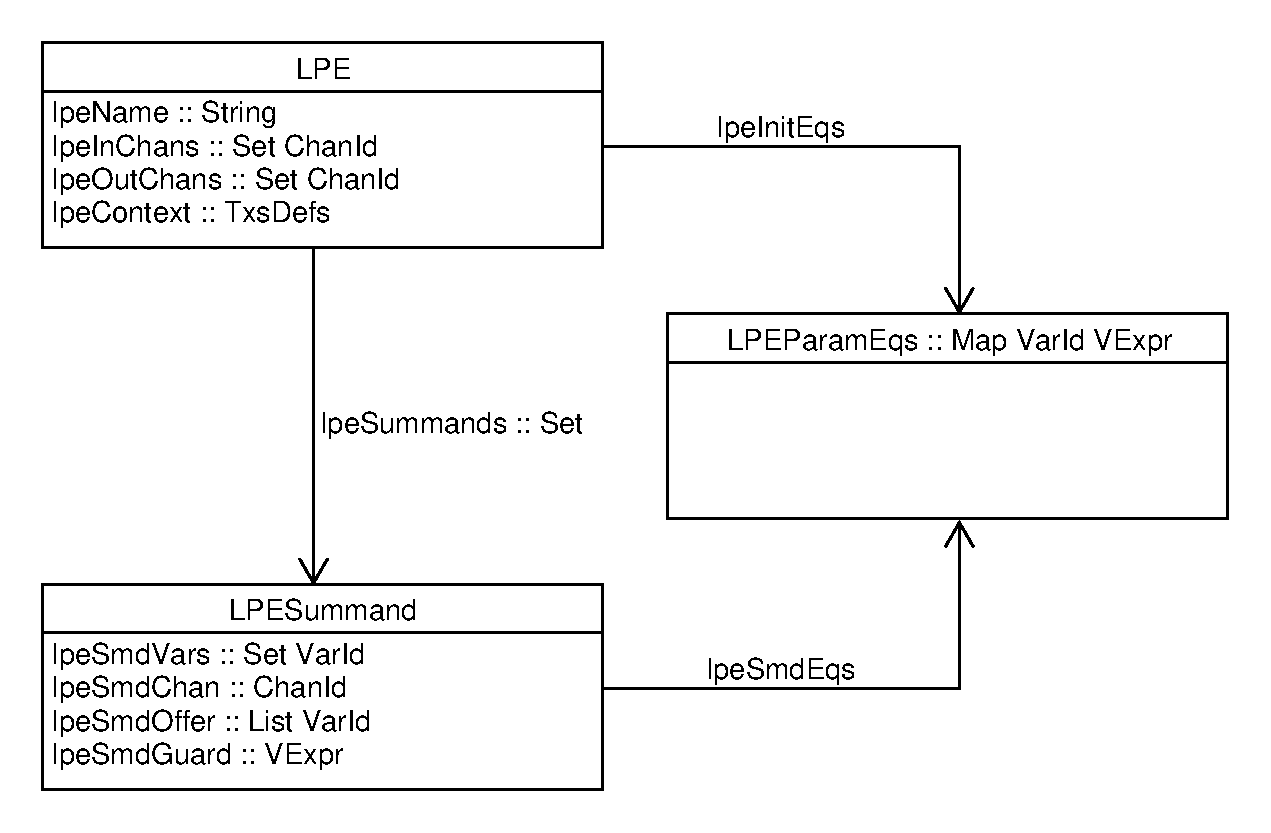
\includegraphics[width=0.7\linewidth]{images/lpe-types}
\caption{LPE data structure.}
\label{lpedatastructure:fig}
\end{center}
\end{figure}

The main data type is \texttt{LPE}.
This type primarily contains information about the \txs{} process in restricted LPE form (see \ref{restrictedlpeform}):
\begin{itemize}
\item The name of the LPE process is \texttt{lpeName};
\item The summands that form the body of the LPE process; and
\item The sorts of the data parameters of the LPE process are contained in \texttt{lpeInitEqs} as well as how each data parameter is initialized.
\end{itemize}

Because the LPE process is always instantiated with the same channels in the same order, the \texttt{LPE} type only has to track which channels are input channels (\texttt{lpeInChans}) and which channels are output channels (\texttt{lpeOutChans}).
Note that these are single channel identifiers that may have been freshly generated from multi-channel summands or from summands with hidden variables in order to obtain restricted LPE form (see \ref{restrictedlpeform}).
The \texttt{lpeChanMap} defines how channels in the LPE data structure are converted back to the original channels; it is therefore the implementation of $\Omega_I$ and $\Omega_O$.

The \texttt{LPE} type also stores some circumstantial information in \texttt{lpeContext}.
This is a library of \txs{} type and function definitions that has been copied directly from the original \txs{} model specification.
It is used to validate instances of the \texttt{LPE} type, to generate default values of a specific sort, and more.

Finally, the \texttt{LPESummand} type only contains information about a specific summand: \texttt{lpeSmdChan} is the channel over which it communicates; \texttt{lpeSmdOffers} are the communication variables (including variables that originally were hidden variables); and the \texttt{lpeSmdEqs} map defines which expressions are used to assign new values to the parameters of the LPE after the application of the summand.

\section{Summand elements} \label{summandelements}

To formally reference the elements of $s_i$ -- the $i$th summand of restricted LPE $P$ -- the following definition is used:
\begin{align*}
s_i = C_i \; \texttt{?} \; x_i(1) \; \cdots{} \; \texttt{?} \; x_i(m_i) \; [[g_i]] \text{ \texttt{>->} } P(v_i(p_1), \cdots{}, v_i(p_k))
\end{align*}

where

\begin{itemize}
\item $C_i$ is the name of the channel over which summand $s_i$ communicates;
\item $m_i \geq 0$ is the number of variables that summand $s_i$ uses to communicate over channel $C_i$;
\item $x_i(j)$ is the $j$th variable that summand $s_i$ uses locally (communication variables first, followed by hidden variables);
\item $g_i$ is the guard of summand $s_i$ (the only free variables in this expression must be parameters of $P$, communication variables of summand $s_i$, or hidden variables of summand $s_i$);
\item $p_1, \cdots{}, p_k$ are the parameters of $P$, of which there are $k \geq 0$;
\item $v_i(p)$ is an expression that defines the new value of parameter $p$ of $P$ after the application of summand $s_i$ (the only free variables in this expression must be LPE parameters, communication variables of summand $s_i$, or hidden variables of summand $s_i$).
\end{itemize}


\chapter{LPE operations}

\section{Introduction}

This section gives an overview of the available LPE operations in \txs{} and how they are used.

\section{Usage}

The \texttt{lpeop} command has 3 space-separated arguments. In order, these arguments are:

\begin{itemize}
\item A chain of LPE operations.
LPE operations are represented by their name, such as \texttt{cstelm} or \texttt{loop}.
These names are separated by the symbol \texttt{->}.

LPE operations in the chain are executed from left to right, passing their output to the next LPE operation as input.
If a problem occurs, the process ends immediately.
Otherwise, the final output model is saved as a new model.
\item The name of the input model.
The input model should be in restricted model form (see \ref{sec:restrictedmodelform}).
\item A base name \textit{base} for generated output.
The name is primarily used for the output model (if any), which is in restricted model form.
However, LPE operations may adopt the name for their own purposes.
The \texttt{export} operation, for example, will create a file by that name with the \texttt{.txs} extension.

It is possible to use the \texttt{\%i} token in the base name.
This will insert the current counter value into the name.
Use the \texttt{inc} command to increase the counter (which starts at 1).
\end{itemize}

\section{Operations}

\subsection{Basic operations}

Table~\ref{tab:basiclpeops} gives an overview of the basic LPE operations.

\begin{table}[!ht]
\begin{center}
\begin{tabularx}{\linewidth}{l|X|}
\textbf{Operation} & \textbf{Description} \\ \hline
\texttt{stop} & End the chain of operations immediately. \\ \hline
\texttt{show} & Print the input LPE to the terminal. \\ \hline
\texttt{show*} & Same as \texttt{show}, but the output is compilable \txs{} code, and identifiers in the output have been shortened for readability. \\ \hline
\texttt{export} & Save the input LPE to \textit{base}\texttt{.txt}. \\ \hline
\texttt{export*} & Same as \texttt{export}, but the output is compilable \txs{} code, and identifiers in the output have been shortened for readability. \\ \hline
\texttt{loop} & If the input LPE has not been encountered before, restart from the most recent \texttt{start} command, or from the first operation if no \texttt{start} command has been encountered yet. \\ \hline
\texttt{loop*}$N$ & Same as \texttt{loop}, but the number of restarts is limited to $N$. \\ \hline
\texttt{start} & Set the location where the command chain should continue when looping. \\ \hline
\texttt{inc} & Increase the counter that can be used in \textit{base}. \\ \hline
\end{tabularx}
\caption{Basic LPE operations.}
\label{tab:basiclpeops}
\end{center}
\end{table}

\subsection{Analysis operations}

Table~\ref{tab:lpeanalysisops} gives an overview of the LPE analysis operations.

\begin{table}[!ht]
\begin{center}
\begin{tabularx}{\linewidth}{l|X|}
\textbf{Operation} & \textbf{Description} \\ \hline
\texttt{isdet} & Return the input LPE after assessing whether it is deterministic. May yield false negatives. \\ \hline
\texttt{mcrl2} & Convert the current LPE to an \mcrl{} specification (so that \mcrl{} can analyze it), and save it to \textit{base}\texttt{.mcrl2}. \\ \hline
\texttt{confcheck} & Perform a confluence analysis on the input LPE, and return the input LPE in which confluent \texttt{ISTEP}s have been renamed to \texttt{CISTEP}s. \\ \hline
\end{tabularx}
\caption{LPE analysis operations.}
\label{tab:lpeanalysisops}
\end{center}
\end{table}

\subsection{Rewrite operations}

Table~\ref{tab:lperewriteops} gives an overview of the LPE rewrite operations.
Table~\ref{tab:lperewriteopsprops} shows which equivalence is preserved by each rewrite operation.

\begin{table}[!ht]
\begin{center}
\begin{tabularx}{\linewidth}{l|X|}
\textbf{Operation} & \textbf{Description} \\ \hline
\texttt{clean} & Remove summands of which it can be established that there already exists an equivalent instance in the LPE from the input LPE; and remove summands of which it can be established via symbolic reachability that they cannot be reached from the input LPE. \\ \hline
\texttt{cstelm} & Remove parameters of which it can be established that their value never changes from the input LPE. \\ \hline
\texttt{parelm} & Remove parameters of which it can be established that their value is never used from the input LPE. \\ \hline
\texttt{parreset} & Set parameters of which it can be established via symbolic reachability that their value is no longer used after a specific summand to a default value in the process instantiation of that summand. \\ \hline
\texttt{datareset} & Set parameters of which it can be established via control-flow analysis that their value is no longer used after a specific summand to a default value in the process instantiation of that summand. \\ \hline
\texttt{confelm} & Rewrite the input LPE so that confluent \texttt{ISTEP} summands are prioritized. \\ \hline
\texttt{istepelm} & Rewrite the input LPE so that \texttt{ISTEP} channels no longer occur. \\ \hline
\texttt{det} & \textit{Experimental.} Rewrite the input LPE in an attempt to reduce non-determinism. By design, \texttt{det} does not generally remove all non-determinism in one execution because it may not terminate (so use with \texttt{loop}). \\ \hline
\texttt{uguard} & \textit{Experimental.} Search for underspecified summands and remove them from the input LPE. \\ \hline
\end{tabularx}
\caption{LPE rewrite operations.}
\label{tab:lperewriteops}
\end{center}
\end{table}

\begin{table}[!ht]
\begin{center}
\begin{tabularx}{\linewidth}{X|c|c|c|c|}
\textbf{Operation} & \textbf{u-ioco} & \textbf{br. bis.} & \textbf{strong bis.} & \textbf{state sp. equiv.} \\ \hline
\texttt{clean} & Yes & Yes & Yes & Yes \\ \hline
\texttt{cstelm} & Yes & Yes & Yes & Yes\footnote{\label{statevectors}Only change is that state vectors may be smaller.} \\ \hline
\texttt{parelm} & Yes & Yes & Yes & No \\ \hline
\texttt{parreset} & Yes & Yes & Yes & No \\ \hline
\texttt{datareset} & Yes & Yes & Yes & No \\ \hline
\texttt{confelm} & Yes & Yes & No & No \\ \hline
\texttt{istepelm} & Yes & Yes & No & No \\ \hline
\texttt{det} & Yes & Yes & Yes & No \\ \hline
\texttt{uguard} & Yes & No & No & No \\ \hline
\end{tabularx}
\caption{LPE rewrite operations.}
\label{tab:lperewriteopsprops}
\end{center}
\end{table}




\chapter{clean}

\section{Introduction}

An LPE may contain redundant information, for example because some of its summands contain all behavior of other summands or because some of its summands will never be (or become) enabled.
Obviously, such summands can be removed without hesitation, which may result in a speedup in other computations in which the LPE is input.

The \texttt{clean} command attempts to detect redundant summands and removes the ones that it finds.
The state space of the LPE is not affected by the changes.

\section{Formal background}

\subsection{Summand containment}

Consider two summands, $s_1$ and $s_2$, defined as

\begin{align*}
s_i &= C_i(1) \;|\; \cdots{} \;|\; C_i(n_i) \; [[g_i]] \text{ \texttt{>->} } P(p_1 = f_i(p_1), \cdots{}, p_m = f_i(p_m)) \\
C_i(x) &= c_i(x) \text{ \texttt{?} } v_i(x,1) \cdots{} \text{ \texttt{?} } v_i(x,k_i(x))
\end{align*}

where

\begin{itemize}
\item $C_i(1) \;|\; \cdots{} \;|\; C_i(n_i)$ are the channel communications used in summand $s_i$;
\item $n_i \geq 0$ is the number of channels over which summand $s_i$ communicates;
\item $g_i$ is the guard of summand $s_i$ (the only free variables in this expression must be LPE parameters or communication variables of summand $s_i$);
\item $P$ is the LPE to which summand $s_i$ belongs;
\item $p_1, \cdots{}, p_m$ are the parameters of the LPE, of which there are $m \geq 0$;
\item $f_i(p)$ is an expression that defines the new value of LPE parameter $p$ after the application of summand $s_i$ (the only free variables in this expression must be LPE parameters or communication variables of summand $s_i$);
\item $c_i(x)$ is the name of the $x$th channel over which summand $s_i$ communicates;
\item $v_i(x,y)$ is the variable that summand $s_i$ uses to communicate the $y$th value of the $x$th channel;
\item $k_i(x)$ is the number of variables that summand $s_i$ uses to communicate over the $x$th channel.
\end{itemize}

Summand $s_1$ is said to \emph{contain} $s_2$ if these two conditions hold:

\begin{itemize}
\item $s_1$ and $s_2$ must communicate over exactly the same channels with exactly as many channel variables; that is,
\begin{align*}
n_1 = n_2 \land \forall x \in [1, \cdots{}, n_1] \;.\; c_1(x) = c_2(x) \land k_1(x) = k_2(x)
\end{align*}

\item Given the previous condition, define
\begin{align*}
n &= n_1 = n_2 \\
k(x) &= k_1(x) = k_2(x) \text{ for all } x \in [1, \cdots{}, n]
\end{align*}

and define, in particular, the mapping
\begin{align*}
V = [v_2(x,y) \rightarrow v_1(x,y) \;|\; x \in [1, \cdots{}, n], y \in [1, \cdots{}, k(x)]]
\end{align*}

The following conditions must also hold:
\begin{align*}
g_2[V] &\rightarrow g_1 \\
f_1(p) = f_2(p)[V] &\leftrightarrow \text{\textit{True}} \text{ for all } p \in [p_1, \cdots{}, p_m]
\end{align*}

The first condition demands that whenever $s_2$ is enabled, $s_1$ must also be enabled; consequently, $s_1$ is `always ready' to perform the same behavior as $s_2$.
The second condition demands that the state after the application of $s_1$ is the same as the state after the application of $s_2$, regardless of the values of communication variables and LPE parameters.
\end{itemize}

Note that $s_1$ could contain all behavior of $s_2$ without these two conditions being true (we under-approximate by tolerating false negatives)!

\subsection{Summand reachability}

Consider all possible pairs of summands of the LPE (including symmetric pairs).
Of a given summand pair $(s, t)$, let $s$ be a \emph{possible predecessor} of $s$ if the following equation is satisfiable:
\begin{align*}
c_s \land {c_t}[p \rightarrow q(p) \;|\; p \in P][q(p) \rightarrow v_s(p) \;|\; p \in P]
\end{align*}

where

\begin{itemize}
\item $c_s$ and $c_t$ are the guards of summands $s$ and $t$, respectively;
\item $P$ is the set of all LPE parameters;
\item $q(p)$ is a bijective function that relates LPE parameter $p$ to a fresh variable;
\item $v_s(p)$ is the expression that defines the new value of LPE parameter $p$ after the application of summand $s$.
\end{itemize}

The fresh variables of the bijective function $q(p)$ are necessary to distinguish LPE parameters before and after the application of summand $s$ (if $p$ is the LPE parameter before, then $q(p)$ is the LPE parameter after).

A summand $t$ is said to be \emph{reachable} if at least one of these two condition holds:

\begin{itemize}
\item Summand $t$ is enabled in the initial state of the LPE.
Formally, if the LPE is initialized as

\begin{align*}
P(p_1 = v_I(p_1), \cdots{}, p_m = v_I(p_m))
\end{align*}

where

\begin{itemize}
\item $P$ is the LPE to which summand $t$ belongs;
\item $p_1, \cdots{}, p_m$ are the parameters of the LPE, of which there are $m \geq 0$;
\item $v_I(p)$ is a closed expression that defines the initial value of LPE parameter $p$;
\end{itemize}

then

\begin{align*}
c_t[p \rightarrow v_I(p) \;|\; p \in P]
\end{align*}

must be satisfiable.

\item There exists at least one other summand $s$ in the same LPE that is a possible predecessor of $t$.
It is \emph{not} sufficient if the only possible predecessor of $t$ is $t$ itself!
\end{itemize}

\section{Implementation}

\subsection{Algorithm}

The algorithm consists of 2 phases.

In the first phase, the algorithm does a pairwise comparison of all summands of the LPE.
If it discovers that some summand $s_1$ contains another summand $s_2$, it removes $s_2$ from the LPE.

In the second phase, the algorithm starts by determining which summands are reachable in the initial state of the LPE (the first condition for reachability in the previous section).
This becomes the initial value of the set $X$.
Then, until a fixpoint is reached, to $X$ all summands are added of which there exists a possible predecessor in $X$.
The output LPE of the algorithm contains all summands that are in the fixpoint of $X$.

\subsection{Complexity}

The complexity of the algorithm is $O(n^2)$, where $n$ is the number of summands of the input LPE.

\section{Example TODO}

Consider the following LPE:

\begin{lstlisting}
//Process definition:
PROCDEF example[A :: Int, B](x, y :: Int)
  = A ? i [[x==0]] >-> example[A, B](1, i)
  + A ? i [[x==1 && i==y]] >-> example[A, B](2, y)
  + B [[x==2]] >-> example[A, B](3, y)
  + B [[x==3]] >-> example[A, B](0, y)
  ;

//Initialization:
example[A, B](0, 0);
\end{lstlisting}

Finding the successors of each summand is easy: each summand has exactly one successor, namely the next one, except in case of the fourth summand, where the first summand is the successor.

It is also obvious that $x$ will always be in $R_s$ for each summand $s$, because each summand uses $x$ in its guard.

Process parameter $y$ will always be in $R_{s_1}$, where $s_1$ is the first summand, because $y$ is used in the guard of $s_1$'s successor (the second summand).
After a few iterations, however, $y$ is removed from $R_{s_2}$ to $R_{s_4}$.
This means that $y$ is assigned a default value in the corresponding summands.
Depending on the mood of the SMT solver, this could give

\begin{lstlisting}
//Process definition:
PROCDEF example[A :: Int, B](x, y :: Int)
  = A ? i [[x==0]] >-> example[A, B](1, i)
  + A ? i [[x==1 && i==y]] >-> example[A, B](2, 0)
  + B [[x==2]] >-> example[A, B](3, 0)
  + B [[x==3]] >-> example[A, B](0, 0)
  ;

//Initialization:
example[A, B](0, 0);
\end{lstlisting}





\chapter{cstelm}

\section{Introduction}

An LPE may have parameters that do not change value throughout the state space of that process.
These parameters are essentially \emph{constant}.
Removing constant parameters results in a smaller state vector (which may improve performance), but otherwise the state space of an LPE remains the same.

Constants can be safely removed from a process as follows:
\begin{itemize}
\item Substitute references to a constant parameter by the initial (explicit) value of that parameter;
\item Remove the constant from the process parameter list.
\end{itemize}

\section{Algorithm}

The algorithm consists of the following steps \cite{groote2001computer}:

\begin{enumerate}

\item Mark all LPE parameters as `constant'.

\item Let $P$ be the set of all LPE parameters that are marked as `constant'.
Define a substitution $\rho = [p \rightarrow v_I(p) \;|\; p \in P]$, where $v_I(p)$ gives the initial value of LPE parameter $p$.

\item Consider each summand $s$ of the LPE.
Construct an equation $c_s \rightarrow p = v_s(p)$ for all $p \in P$, where $c_s$ is the guard of $s$ and where $v_s(p)$ is the expression that defines the value of LPE parameter $p$ after the application of summand $s$, and apply the substitution $\rho$ to it.
(This gives $(c_s \rightarrow p = v_s(p))[\rho] \Leftrightarrow {c_s}[\rho] \rightarrow v_I(p) = v_s(p)[\rho]$.)

If the obtained equation is a tautology (that is, if its negation is unsatisfiable) for all $s$, $p$ remains marked as `constant'; otherwise, unmark $p$.

\item Repeat the previous two steps until the fixpoint of $P$ is reached.
Then remove all LPE parameters that are still marked as `constant' from the LPE, substituting references to those parameters by their initial values.

\end{enumerate}

\section{Example TOCHECK}

Consider the following LPE:

\begin{lstlisting}
//Process definition:
PROCDEF example[A](x, y, z :: Int)
  = A [[z = 2]] >-> example[A](z-1, 1, 2)
  + A >-> example[A](y, x, x+y)
  + A >-> example[A](1, x, z+1)
  ;

//Initialization:
example[A](1, 1, 2);
\end{lstlisting}

First, $\rho = [ x \rightarrow 1, y \rightarrow 1, z \rightarrow 2 ]$.

We must check the following equations:

\begin{align*}
(z = 2 \rightarrow x = z-1)[\rho] &\Leftrightarrow (2 = 2 \rightarrow 1 = 2-1) \Leftrightarrow \textit{true} \\
(z = 2 \rightarrow y = 1)[\rho] &\Leftrightarrow (2 = 2 \rightarrow 1 = 1) \Leftrightarrow \textit{true} \\
(z = 2 \rightarrow z = 2)[\rho] &\Leftrightarrow (2 = 2 \rightarrow 2 = 2) \Leftrightarrow \textit{true} \\
(x = y)[\rho] &\Leftrightarrow (1 = 1) \Leftrightarrow \textit{true} \\
(y = x)[\rho] &\Leftrightarrow (1 = 1) \Leftrightarrow \textit{true} \\
(z = x+y)[\rho] &\Leftrightarrow (2 = 1+1) \Leftrightarrow \textit{true} \\
(x = 1)[\rho] &\Leftrightarrow (1 = 1) \Leftrightarrow \textit{true} \\
(y = x)[\rho] &\Leftrightarrow (1 = 1) \Leftrightarrow \textit{true} \\
(z = z+1)[\rho] &\Leftrightarrow (2 = 2+1) \Leftrightarrow \textit{false} \\
\end{align*}

The last equation is not a tautology, and so $z$ is unmarked.

The new value of $\rho$ is $[ x \rightarrow 1, y \rightarrow 1 ]$.

\clearpage
The equations are now the following:

\begin{align*}
(z = 2 \rightarrow x = z-1)[\rho] &\Leftrightarrow (z = 2 \rightarrow 1 = z-1) \Leftrightarrow \textit{true} \\
(z = 2 \rightarrow y = 1)[\rho] &\Leftrightarrow (z = 2 \rightarrow 1 = 1) \Leftrightarrow \textit{true} \\
(x = y)[\rho] &\Leftrightarrow (1 = 1) \Leftrightarrow \textit{true} \\
(y = x)[\rho] &\Leftrightarrow (1 = 1) \Leftrightarrow \textit{true} \\
(x = 1)[\rho] &\Leftrightarrow (1 = 1) \Leftrightarrow \textit{true} \\
(y = x)[\rho] &\Leftrightarrow (1 = 1) \Leftrightarrow \textit{true} \\
\end{align*}

All of the equations above are tautologies, and so $x$ and $y$ remain marked.
Removing the marked parameters from the LPE gives

\begin{lstlisting}
//Process definition:
PROCDEF example[A](z :: Int)
  = A [[z==2]] >-> example[A](2)
  + A >-> example[A](2)
  + A >-> example[A](z+1)
  ;

//Initialization:
example[A](2);
\end{lstlisting}

Obviously, more simplification is possible.


\input{parelm}
\input{parreset}
\input{datareset}
\input{confcheck}
\input{confelm}
%\chapter{istepelm}




%\input{mcrl2}
\chapter{isdet} \label{isdet}

\section{Introduction}

The \texttt{isdet} command checks whether the specified LPE is deterministic.
The command may yield false negatives.

\section{Formal background}

\subsection{Summand determinism}

Consider two summands, $s_\alpha$ and $s_\beta$, and reference their elements conform \ref{summandelements}.

Summands $s_\alpha$ and $s_\beta$ are said to be \emph{deterministic} if one of these conditions holds:

\begin{itemize}
\item $s_\alpha$ and $s_\beta$ are the same summand; that is, $s_\alpha = s_\beta$.

\item $s_\alpha$ and $s_\beta$ communicate over different channels:
\begin{align*}
C_\alpha \neq C_\beta \land (C_\alpha \in \{\istep{}, \cistep{}\} \not\leftrightarrow C_\beta \in \{\istep{}, \cistep{}\})
\end{align*}

\item $s_\alpha$ and $s_\beta$ communicate with different numbers of communication variables; that is, $m_\alpha \neq m_\beta$.

\item $s_\alpha$ and $s_\beta$ are never simultaneously enabled, or $s_\alpha$ and $s_\beta$ always lead to the same next state.
In order to determine this, check if
\begin{align*}
g_\alpha[X_\beta] \land g_\beta \rightarrow \bigwedge\limits_{j=1}^{k} v_\alpha(p_j)[X_\beta] = v_\beta(p_j)
\end{align*}

is a tautology, where $X_\beta$ is defined as
\begin{align*}
X_{\beta} &= [x_\alpha(j) \rightarrow x_\beta(j) \;|\; 1 \leq j \leq \text{min}(m_\alpha, m_\beta)]
\end{align*}
\end{itemize}

Note that this approach is \emph{not} guaranteed to correctly recognize that two summands are deterministic (false negatives are tolerated)!

\section{Algorithm}

The algorithm invoked by the \texttt{isdet} command checks for all pairs of different summands whether the first summand is deterministic with the second summand (see the previous section).
The algorithm yields \textbf{true} if and only if this is the case for all summand pairs.

\section{Example}

Consider the following LPE:

\begin{lstlisting}
//Process definition:
PROCDEF example[A :: Int](x, y :: Int)
  = A ? i [[x==0 /\ i>=0 /\ i<=5]] >-> example[A](1, 0)
  + A ? i [[y==0 /\ i>=5 /\ i<=9]] >-> example[A](0, 1)
  ;

//Initialization:
example[A](0, 1);
\end{lstlisting}

Consider the two summands, calling the first $s_1$ and the second $s_2$.

The first three conditions for detecting determinism are false.

For the fourth condition, the antecedent is
\begin{align*}
g_1[X_2] \land g_2 &\Leftrightarrow (\texttt{x} = 0 \land \texttt{i} \geq 0 \land \texttt{i} \leq 5)[\texttt{i} \rightarrow \texttt{i}] \land (\texttt{y} = 0 \land \texttt{i} \geq 5 \land \texttt{i} \leq 9) \\
&\Leftrightarrow \texttt{x} = 0 \land \texttt{y} = 0 \land \texttt{i} = 5
\end{align*}

Given the antecedent, the conclusion must hold.
This is not the case:
\begin{align*}
v_1(\texttt{x})[X_2] = 1[\texttt{i} \rightarrow \texttt{i}] = 1 \neq 0 = v_2(\texttt{x}) \\
v_1(\texttt{y})[X_2] = 0[\texttt{i} \rightarrow \texttt{i}] = 0 \neq 1 = v_2(\texttt{y}) \\
\end{align*}

$s_1$ is therefore \emph{not} deterministic with $s_2$.

Changing the LPE to

\begin{lstlisting}
//Process definition:
PROCDEF example[A :: Int](x, y :: Int)
  = A ? i [[x==0 /\ i>=0 /\ i<=4]] >-> example[A](1, 0)
  + A ? i [[y==0 /\ i>=5 /\ i<=9]] >-> example[A](0, 1)
  ;

//Initialization:
example[A](0, 1);
\end{lstlisting}

will result in an antecedent that is false; therefore, $s_1$ is deterministic with $s_2$.


\chapter{det}

\section{Introduction}

Non-determinism in an LPE can have a strong impact on the performance of exploring its state space.
Preferably, an LPE should therefore be completely deterministic.
Unfortunately, there are no determinization methods known for symbolic models such as LPEs.

The \texttt{det} command described in this section is only a naive attempt at LPE determinization: it looks for two summands that are non-deterministic (see \ref{isdet}), and then rewrites the LPE so that these summands have become deterministic.
This may mean that the entire LPE has become deterministic, but more typically the non-determinism will have moved to a different part of the LPE.

The \texttt{det} command is intended to be repeated in the hope that non-determinism eventually disappears from the LPE.
It is definitely possible that this may never happen!
It is also likely that the LPE will grow very large; it is therefore advised to symbolically reduce the LPE using other LPE operations after each application of \texttt{det}.

\section{Algorithm}

Let the input LPE model be $M$ and the underlying LPE be $P$, and let two summands of $P$, $s_\alpha$ and $s_\beta$, be non-deterministic (see \ref{isdet}).
Elements of $s_\alpha$ and $s_\beta$ are referenced conform \ref{summandelements}.
Define
\begin{align*}
C_{\alpha,\beta} &= C_\alpha = C_\beta \\
m_{\alpha,\beta} &= m_\alpha = m_\beta \\
X_\alpha &= [ x_\beta(j) \rightarrow x_\alpha(j) \;|\; 1 \leq j \leq m_{\alpha,\beta} ] \\
X_\beta &= [ x_\alpha(j) \rightarrow x_\beta(j) \;|\; 1 \leq j \leq m_{\alpha,\beta} ]
\end{align*}

and let $y(j)$ be a bijective function that yields fresh variables for $1 \leq j \leq m_{\alpha,\beta}$.

The \texttt{det} algorithm follows these steps:

\begin{enumerate}
\item Create a new LPE $P'$ with the same parameters as $P$, but without any summands.
Create a new LPE model $M'$ that has the same definition as $M$, except that its references to $P$ have been replaced by references to $P'$.

\item Add a new, fresh parameter $f$ of type \texttt{Bool} to $P'$.
Where $M'$ instantiates $P'$, initialize $f$ with $\textbf{false}$.

\item Add a new, fresh parameter $Y$ to $P'$, which is a substitution from variables to values -- in practice, this is implemented with multiple parameters and/or a data hierarchy.
Where $M'$ instantiates $P'$, initialize $Y$ with $[]$.

\item Add to $P'$ each summand $s_i, i \neq \alpha, \beta$ of $P$ after changing the guard of $s_i$ from $g_i$ to $\neg f \land g_i$.

\item Add to $P'$ two new summands ${s_\alpha}'$ and ${s_\beta}'$ that are defined as
\begin{align*}
{s_\alpha}' = C_{\alpha,\beta} \; \texttt{?} \; x_\alpha(1) \; &\cdots{} \; \texttt{?} \; x_\alpha(m_{\alpha,\beta}) \; [[\neg f \land g_\alpha \land \neg g_\beta[X_\alpha]]] \\
&\texttt{>->} \; P(v_\alpha(p_\alpha), \cdots{}, v_\alpha(p_k), \textbf{false}, []) \\
{s_\beta}' = C_{\alpha,\beta} \; \texttt{?} \; x_\beta(1) \; &\cdots{} \; \texttt{?} \; x_\beta(m_{\alpha,\beta}) \; [[\neg f \land \neg g_\alpha[X_\beta] \land g_\beta]] \\
&\texttt{>->} \; P(v_\beta(p_\alpha), \cdots{}, v_\beta(p_k), \textbf{false}, [])
\end{align*}

\item Add to $P'$ a new summand ${s_{\alpha,\beta}}'$ that is defined as
\begin{align*}
{s_{\alpha,\beta}}' &= C_{\alpha,\beta} \; \texttt{?} \; x_\alpha(1) \; \cdots{} \; \texttt{?} \; x_\alpha(m_{\alpha,\beta}) \; [[\neg f \land g_\alpha \land g_\beta[X_\alpha]]] \\
&\texttt{>->} \; P(p_1, \cdots{}, p_k, \textbf{true}, [y(1) \rightarrow x_\alpha(1), \cdots{}, y(m_{\alpha,\beta}) \rightarrow x_\alpha(m_{\alpha,\beta})])
\end{align*}

\item For $i \in \{\alpha, \beta\}$ and for each possible successor $s_\gamma$ of $s_i$ (see \ref{possiblesuccessors}) in $P$, add to $P'$ a new summand ${s_\gamma}'$ that is defined as
\begin{align*}
{s_\gamma}' = C_\gamma \; \texttt{?} \; x_\gamma(1) \; &\cdots{} \; \texttt{?} \; x_\gamma(m_\gamma) \; [[f \land g_\gamma[Y_i]]] \\
&\texttt{>->} \; P(v_\gamma(p_1)[Y_i], \cdots{}, v_\gamma(p_k)[Y_i], \textbf{false}, [])
\end{align*}

where
\begin{align*}
Y_i &= [ p_j \rightarrow v_i(p_j)[\overline{Y_i}][Y] \;|\; 1 \leq j \leq k ] \\
\overline{Y_i} &= [x_i(1) \rightarrow y(1), \cdots{}, x_i(m_{\alpha,\beta}) \rightarrow y(m_{\alpha,\beta})]
\end{align*}

\end{enumerate}

Intuitively, the specific non-deterministic behavior of summands $s_\alpha$ and $s_\beta$ is preserved by summand ${s_{\alpha,\beta}}'$, while summands ${s_\alpha}'$ and ${s_\beta}'$ cover the deterministic behavior.
The $f$ parameter indicates that the process has just taken the non-deterministic action of ${s_\gamma}'$, and the $Y$ parameter contains the exact communication values of that action.

If $f$ is \textbf{false}, $P'$ has the same behavior as $P$ because the summands that are created in steps 4 to 6.
If $f$ is \textbf{true}, $P'$ also has the same behavior as $P$, but in such a way that the changes of summands $s_\alpha$ and $s_\beta$ are applied retroactively.

\section{Example}

Consider the following LPE:

\begin{lstlisting}
//Process definition:
PROCDEF example[A :: Int, B, C](x, y :: Int)
  = A ? i [[x==0 /\ i>=0 /\ i<=5]] >-> example[A, B, C](1, i+1)
  + A ? i [[x==0 /\ i>=5 /\ i<=9]] >-> example[A, B, C](1, i-1)
  + B [[x==1 /\ y<=4]] >-> example[A, B, C](0, 0)
  + C [[x==1 /\ y>=5]] >-> example[A, B, C](0, 0)
  ;

//Initialization:
example[A, B, C](0, 0);
\end{lstlisting}

Consider the first two summands, calling the first $s_1$ and the second $s_2$.
These summands are non-deterministic.

Applying the steps of the \texttt{det} algorithm causes the following changes:

\begin{enumerate}
\item A new LPE model $M'$ and new LPE $P'$ are created.
\item $P'$ is extended with a new parameter $\texttt{f}$.
\item $P'$ is extended with a new parameter $\texttt{z}$ (a singleton substitution).
\item The \texttt{B} and \texttt{C} summands of the input LPE are added with modified guards.
\item Based on $s_1$ and $s_2$, summands ${s_1}'$ and ${s_2}'$ are created and added.
\item Based on $s_1$ and $s_2$, summand ${s_{1, 2}}'$ is created and added.
\item The possible successors of $s_1$ and $s_2$ are the \texttt{B} and \texttt{C} summands of the input LPE, which results in 2 new \texttt{B} summands and 2 new \texttt{C} summands.
\end{enumerate}

This gives the following output LPE:

\begin{lstlisting}
PROCDEF example'[A :: Int, B, C](x, y :: Int, f: Bool, z: Int)
  = B [[not(f) /\ x==1 /\ y<=4]]
          >-> example'[A, B, C](0, 0, false, 0)
  + C [[not(f) /\ x==1 /\ y>=5]]
          >-> example'[A, B, C](0, 0, false, 0)
  + A ? i [[not(f) /\ x==0 /\ i>=0 /\ i<5]]
          >-> example'[A, B, C](1, i, false, 0)
  + A ? i [[not(f) /\ x==0 /\ i>5 /\ i<=9]]
          >-> example'[A, B, C](1, i, false, 0)
  + A ? i [[not(f) /\ x==0 /\ i==5]]
          >-> example'[A, B, C](x, y, true, i)
  + B [[f /\ z+1<=4]] >-> example[A, B, C](0, 0, false, 0)
  + B [[f /\ z-1<=4]] >-> example[A, B, C](0, 0, false, 0)
  + C [[f /\ z+1>=5]] >-> example[A, B, C](0, 0, false, 0)
  + C [[f /\ z-1>=5]] >-> example[A, B, C](0, 0, false, 0)
  ;

//Initialization:
example'[A, B, C](0, 0, false, 0);
\end{lstlisting}

The non-determinism has moved to the \texttt{B} and \texttt{C} summands at the bottom.
A subsequent application of the \texttt{clean} command removes one of the \texttt{B} summands at the bottom (because
\begin{align*}
z+1<=4 \rightarrow z-1<=4
\end{align*}

the second \texttt{B} summand \emph{contains} the first) and one of the \texttt{C} summands at the bottom (because
\begin{align*}
z-1>=5 \rightarrow z+1>=5
\end{align*}

the first \texttt{C} summand \emph{contains} the second).
Afterwards, the LPE is completely deterministic.





\chapter{uguard}

\section{Introduction}

\txs{} checks whether or not there is \emph{input-output-conformance} of an implementation with the \emph{underspecified} traces of its specification (u-ioco, see \cite{volpato2013towards}).
In this context, the specification has only to be u-ioco with itself, and it can therefore potentially be rewritten more aggressively than when a models must preserve a stronger equivalence relation.

Unfortunately, there is no information about the traces of a model that can be extracted directly from that model while it is in LPE form.
The \texttt{uguard} command is an attempt to symbolically detect a specific, relatively simple pattern with actions that do not follow the u-ioco definition.
Upon detection, the command adds guards to the LPE to exclude the underspecified actions from the model (hence its name).

\section{Formal background}

\subsection{Summand implication}

Consider two summands, $s_\alpha$ and $s_\beta$, and reference their elements conform \ref{summandelements}.

Summand $s_\alpha$ is said to \emph{imply} $s_\beta$ if these two conditions hold:

\begin{itemize}
\item $s_\alpha$ and $s_\beta$ must communicate over the exact same channel with exactly as many channel variables; that is, $C_\alpha = C_\beta \land m_\alpha = m_\beta$.

\item Define the mapping
\begin{align*}
X_\beta = [x_\alpha(j) \rightarrow x_\beta(j) \;|\; 1 \leq j \leq \text{min}(m_1, m_2)]
\end{align*}

The following condition must be a tautology:
\begin{align*}
g_\alpha[X_\beta] \rightarrow g_\beta
\end{align*}
\end{itemize}

\subsection{Possible input-successors}

Consider all possible pairs of summands $(s_\alpha, s_\beta)$ of the LPE (including symmetric pairs), and reference the elements of $s_\alpha$ and $s_\beta$ conform \ref{summandelements}.
Summand $s_\beta$ is said to be a \emph{possible input-successor} of $s_\alpha$ if $C_\beta$ is an input channel and if the following expression is satisfiable:
\begin{align*}
g_\alpha \land {g_\beta}[p \rightarrow v_\alpha(p) \;|\; p \in P]
\end{align*}

\subsection{Definite input-successors}

Consider all possible pairs of summands $(s_\alpha, s_\beta)$ of the LPE (including symmetric pairs), and reference the elements of $s_\alpha$ and $s_\beta$ conform \ref{summandelements}.
Summand $s_\beta$ is said to be a \emph{definite input-successor} of $s_\alpha$ if $C_\beta$ is an input channel and if the following expression is a tautology:
\begin{align*}
g_\alpha \land {g_\beta}[p \rightarrow v_\alpha(p) \;|\; p \in P]
\end{align*}

\section{Algorithm}

Let the input LPE model be $M$ and the underlying LPE be $P$.
The \texttt{uguard} algorithm follows these steps for all summand pairs $(s_\alpha, s_\beta)$ such that $s_\alpha$ implies $s_\beta$:

\begin{enumerate}
\item Compute $\Delta = (D_\beta \setminus P_\alpha) \cup (D_\alpha \setminus P_\beta)$ where
\begin{itemize}
\item $P_\alpha$ is the set of all possible input-successors of $s_\alpha$;
\item $P_\beta$ is the set of all possible input-successors of $s_\beta$;
\item $D_\alpha$ is the set of all definite input-successors of $s_\alpha$; and
\item $D_\beta$ is the set of all definite input-successors of $s_\beta$.
\end{itemize}

If $\Delta = \emptyset{}$, the \texttt{uguard} algorithm does not make any changes and stops.
Otherwise, it continues.

\item Create a new LPE $P'$ with the same parameters as $P$, but without any summands.
Create a new LPE model $M'$ that has the same definition as $M$, except that its references to $P$ have been replaced by references to $P'$.

\item Add a new, fresh parameter $f$ of type \texttt{Bool} to $P'$.
Where $M'$ instantiates $P'$, initialize $f$ with $\textbf{true}$.

\item For each summand $s_i$ of $P$ -- referencing its elements conform \ref{summandelements} -- add to $P'$ a new summand ${s_i}'$ that is defined as
\begin{align*}
{s_i}' = C_i \; \texttt{?} \; x_i(1) \; &\cdots{} \; \texttt{?} \; x_i(m_i) \; [[\Gamma(s_i) \land g_i]] \\
&\texttt{>->} \; P(v_i(p_1), \cdots{}, v_i(p_k), \Upsilon(s_i))
\end{align*}

where
\begin{align*}
\Gamma(s) = \begin{cases}
f \text{ if } s \in \Delta \\
\textbf{true} \text{ if } s \notin \Delta
\end{cases}
\end{align*}

and
\begin{align*}
\Upsilon(s) = \begin{cases}
\textbf{true} \text{ if } s \neq s_\alpha \land s \neq s_\beta \\
\textbf{false} \text{ if } s = s_\alpha \lor s = s_\beta
\end{cases}
\end{align*}
\end{enumerate}

Intuitively, the algorithm first detects that certain summands are underspecified: they are enabled after a certain action if that action is performed by summand $s_\alpha$, but they are not enabled after that action is performed by summand $s_\beta$.
The algorithm therefore makes it so that the underspecified summands are always disabled after $s_\alpha$ or $s_\beta$ (preserving equivalence up to u-ioco).

\section{Example TODO}

Consider the following LPE:

\begin{lstlisting}
//Process definition:
PROCDEF example[A :: Int, B](x, y :: Int)
  = A ? i [[x==0]] >-> example[A, B](1, i)
  + A ? i [[x==1 && i==y]] >-> example[A, B](2, y)
  + B [[x==2]] >-> example[A, B](3, y)
  + B [[x==3]] >-> example[A, B](0, y)
  ;

//Initialization:
example[A, B](0, 0);
\end{lstlisting}

TODO



\bibliographystyle{plainnat}
\bibliography{biblio}

\end{document}
